\hspace{0.5 cm} În contextul verificării rețelelor neuronale, un benchmark este constituit dintr-o serie de modele neurale testate și specificațiile riguroase ce trebuie satisfăcute pentru a valida corectitudinea și securitatea acestora. 

Modelul neuronal este reprezentat sub forma fișierelor în format .onnx. Aceste fișiere cuprind detaliile arhitecturii modelului, precum straturile rețelei neuronale și parametrii, însă nu includ datele reale de antrenament.

Specificările care sunt supuse verificării sunt reprezentate printr-un set de fișiere în format .vnnlib, care conțin informații esențiale despre rețeaua neuronală. Aceste detalii includ dimensiunile stratului de intrare și de ieșire, precum și intervalul sau domeniul de valori admise pentru activările neuronale.

Benchmark-ul utilizat testează un model deosebit de reațea neuronală care se numește rețea adversară generativă condiționată. Pentru o întelegere mai bună a celui din urmă vom descrie mai întâi ce este o rețea neurală adversară generativă.

\subsection*{GAN}
 \hspace{0.5 cm} Este un model neuronal mai special \cite{GAN} a cărui concept poate fi reprezentat ca un joc între două rețele neuronale distincte adversare sau, altfel spus, între doi jucători. Primul jucator este numit generator, iar al doilea discriminator. 
 
 Rolul generatorului este de a genera date false, bazate pe datele de intrare, care să pară cât mai reale. Generatorul are scopul de a păcăli pe al doilea jucător - discriminantorul. 
 
 Scopul celui de-al doilea jucator este de a determina ce imagini sunt reale și care sunt false, adica realizate de generator. Dacă discriminatorul interpretează corect atunci primește feedback pozitiv, dacă interpretează greșit atunci primește feedback negativ. Discriminatorul are  acces la datele de ce ies din generator, dar si la datele de antrenament.

\begin{figure}[ht]
\centering
{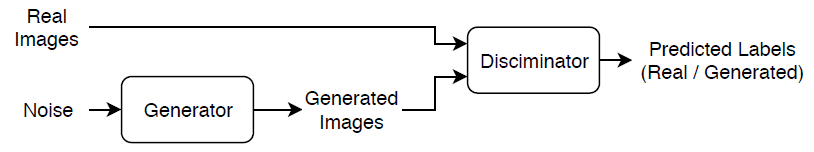
\includegraphics[width=10cm]{imagini/GANarch.png}}
\caption{Mod de lucru al GAN}
\label{modDeLucruGAN}
\end{figure}

Ambii jucători învață și se îmbunătățesc în timp. Generatorul devine mai bun în a crea falsuri convingătoare, iar discriminatorul își îmbunătățește capacitatea de a spune dacă ceva este autentic. De-a lungul timpului, rețeaua ajunge într-un punct în care datele produse de generator vor arăta aproape imposibil de distins de datele din lumea reală.



\subsection*{cGAN}
\hspace{0.5 cm} cGAN, prescurtare de la Conditional Generative Adversarial Networks \cite{CGAN}, ghidează procesul de creare a datelor prin încorporarea unor etichete specificice în GAN. Rețele adversare - generatorul și discriminatorul - se orientează după aceste etichete. 

Generatorul utilizează etichetele pentru a creea date false care imită datele reale și respectă condiția setată. Și la fel ca în modelul GAN, discriminatorul va distinge între datele falsificate produse de generator și datele autentice corespunzătoare condiției date.
\newpage

\begin{figure}[ht]
\centering
{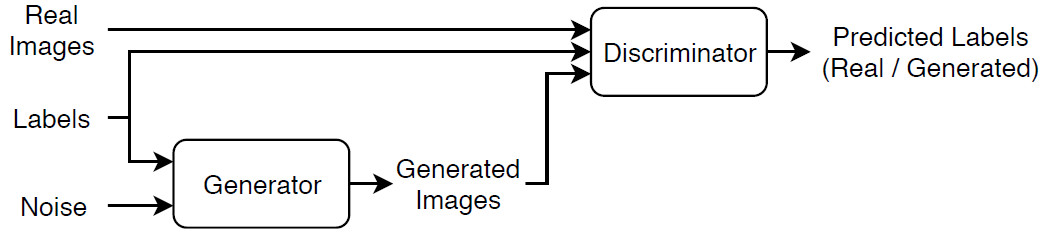
\includegraphics[width=10cm]{imagini/cGANarch.png}}
\caption{Mod de lucru al cGAN}
\label{modDeLucrucGAN}
\end{figure}



De exemplu, să presupunem că ați folosit un spectru larg de imagini cu flori pentru a antrena un GAN capabil să producă imagini false cu flori. Deși puteți folosi modelul dvs. pentru a genera o imagine a unei flori aleatorii, nu îi puteți instrui să creeze o imagine a, de exemplu, a unei lalele sau a unei floarea soarelui.

GAN condiționat (cGAN) ne permite să condiționăm rețeaua cu informații suplimentare, cum ar fi etichetele de clasă. Înseamnă că în timpul antrenamentului, transmitem imagini în rețea cu etichetele lor reale (trandafir, lalele, floarea soarelui etc.) pentru ca aceasta să învețe diferența dintre ele. În acest fel, obținem capacitatea de a cere modelului nostru să genereze imagini cu anumite flori.


\subsection*{cGAN benchmark din vnncomp2023}
Obiectivul \cite{vnncomp2023Chat} modelului neuronal din benchmark-ul cGAN din competiția vnncomp2023 este de a genera imagini ale camerei care conțin un obstacol al vehiculului situat la o anumită distanță în fața vehiculului ego, unde distanța este controlată de condiția distanței de intrare. În figura \ref{imaginiGenerate} sunt ilustrate exemple de imagini create de generatorul din cadrul retelei neurale.

\begin{figure}[ht]
\centering
{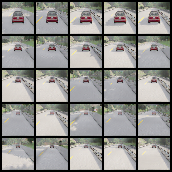
\includegraphics[width=5.75cm]{imagini/obstacle.png}}
\caption{Imagini generate}
\label{imaginiGenerate}
\end{figure}

Generatorul primește două intrări:
\begin{itemize}
\item o condiție de distanță (1-d scalar), între 0 - 1(normalizat de la 0m la 30m). De exemplu, dacă condiția de distanță este 0,5, înseamnă că va fi generată o imagine ce are obstacolul la 15m in fața vehiculului ego.
\item un vector de zgomot care controlează mediul (vector 4-d)
\end{itemize}

Ca și rezultat genratorul returnează o imagine generată.


Discriminatorul consideră imaginea returnată de generator ca și data de intrare și emite ca rezultat urmatoarele:
\begin{itemize}
\item un scor real/fals (1-d scalar), adică dacă trebuie să prezică dacă imaginea a fost realizată de generator sau nu
\item o distanță prezisă (1-d scalar), distanță estimată de discriminant dintre vehiculul ego și vehiculul obstacol
\end{itemize}

\begin{figure}[ht]
\centering
{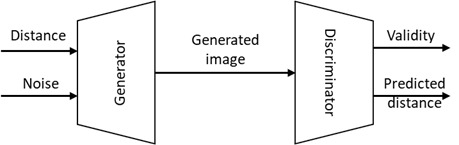
\includegraphics[width=8.5cm]{imagini/cganbench.jpeg}}
\caption{Mod de lucru cGAN benchmark}
\label{cganbench}
\end{figure}

Pentru verificare, am putea combina aceste două componente împreună și am putea stabili specificații de verificare adecvate pentru distanța de intrare, zgomotul de intrare și distanța estimată.

